
\documentclass[twocolumn, amsmath]{revtex4}

\usepackage{graphicx}
%\graphicspath{ {tex_pics/} }


\begin{document}


\title{PHYS 605 Lab \#8} 

\author{Morgan A. Daly}
\author{Evin O'Shea}
\date{\today} 


\maketitle


\section{Introduction and Theory}
\subsection{Purpose}

This lab focused on working with digital ciurcuits. The two digital compontents used were the 555 timer and the nand gate. 

The goal of the first part of the lab was to demonstrate how nand gates work and how they can be used in various ways to create more interesting opertations by combining nand gates. 
the second part of the lab focusxed on the 555 timer. for this part of the lab, they design of the circuit would give a visual queue depending on the output of the 555 timer to demonstrate what the outputwas.



\subsection{Background / Theory}



Digital circuits consist of different high square pulses that can be catagorized as one of two states: high or low; 1 or 0. This type of circuitry is used in a lot of technology because it can send encoded data without error. The error is reduced, because a low andf high pulse can be easily distinguisehed even if there is noise in the signal. This means that the data is only limited by the number of pulses sent.

In the lab, the gropup used LED's to get a visual feedback on the output of the circuit. 
LED's require a minimum voltage across them to light up. This is perfect for digital circuits as the high voltage is over the diode voltage and the low is below it. This means that the LED on is a high coming through and the LED off is as low comming through.

The NAND gate performs the logical operator of "not and". The truth table for this gate is shown below:

\begin{center}
	\begin{ruledtabular}
    \begin{tabular}{ l l l}
	IN$_1$ & IN$_2$ & OUT\\ \colrule
	0 & 0 & 1 \\
	0 & 1 & 1 \\
	1 & 0 & 1 \\
	1 & 1 & 0  \\
\end{tabular}
    \end{ruledtabular}
\end{center}

However, when the inputs are tied together, there are only two cases. This truth table is shown below:

\begin{center}
	\begin{ruledtabular}
    \begin{tabular}{ l l}
	IN & OUT\\ \colrule
	0 & 1 \\
	1 & 0 \\
\end{tabular}
    \end{ruledtabular}
\end{center}

This means that when the inputs are tied together, the NAND gate actually just inverts the signal. The three NAND gates combined in the lab together have their own truth table. For this, we have to consider thatthe two inputs to the first two NAND gates will be inverted. Then, the final NAND gate will take "not and" as shown by the first truth table aboove. However, since these two inputs are inverted, the opposite of each IN will corespond to the same OUT. THe truth table shown below is the equivalent truth table for the three gates:

\begin{center}
	\begin{ruledtabular}
    \begin{tabular}{ l l l}
	IN$_1$ & IN$_2$ & OUT\\ \colrule
	1 & 1 & 1 \\
	1 & 0 & 1 \\
	0 & 1 & 1 \\
	0 & 0 & 0  \\
\end{tabular}
    \end{ruledtabular}
\end{center}

This truth table is equivalent to the truth table of an OR gate. This means the equivalent logical operation for these three gates is "OR".


\begin{figure}[h]
    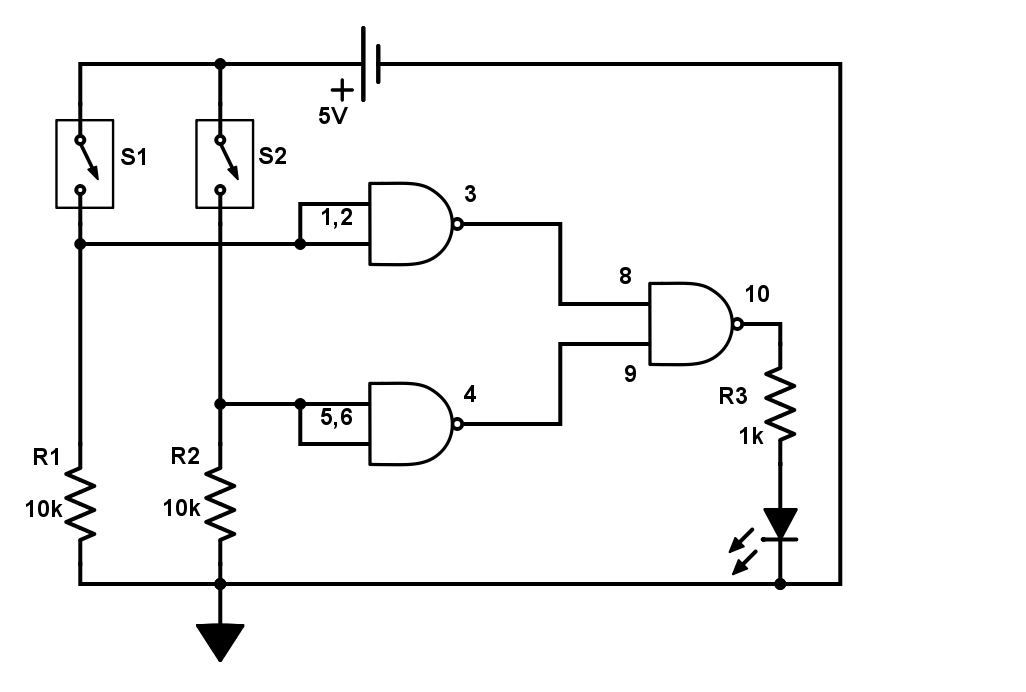
\includegraphics[scale=0.25]{NAND.png}  
    \caption{}
\end{figure}


The resistors used inb this part of the lab were chosen to restrict the current supplied to the NAND gates. Since the supply voltage was 5V, 10k$\Omega$ resistors were used to obtain a 0.5mA current. This is in the rating range of the NAND gates. %something? blah blah sound better etc etc so on and so forth




\begin{figure}[h]
    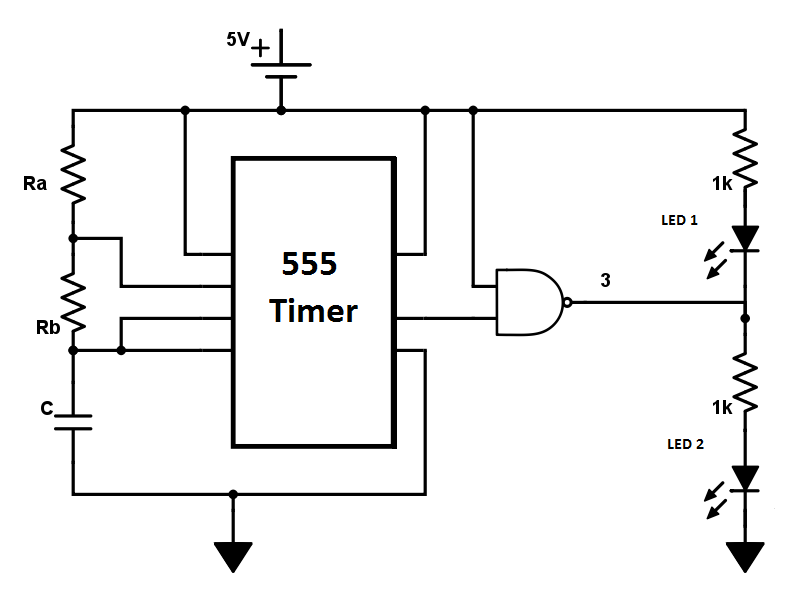
\includegraphics[scale=0.35]{555.png}  
    \caption{}
\end{figure}

\section{Methodology}

%CHECK FIGURE #'s HERE
\begin{enumerate}
    \item Set the circuit up as shown in figure (1). 
    \item Use the switches to change the input coming in and check that the outout is as expected.
    \item Select/calculate values of R$_1$, R$_2$, and C such that the output of the 555 timer will be 2 Hz.
    \item Build the circuit as shown in figure (2).
    \item Test the output of the 555 timer and make sure that it is as expected.
    \item Record the outpuit frequency of the 555 timer.
\end{enumerate}


\section{Results and Analysis}

\subsection{Data}
For part A of the lab, the only data to be recorded was from the visual feedback of the LED's. The logic table shown below demonstrates the lows and highs at various points in the circuit:

\begin{center}
	\begin{ruledtabular}
    \begin{tabular}{ l l l l l l l}
	S1 & S2 & 1,2 & 5,6 & 3,8 & 4,9 & 10, LED \\ \colrule
	0 & 0 & 0 & 0 & 0 & 0 & 0  \\
	0 & 1 & 0 & 1 & 1 & 0 & 1 \\
	1 & 0 & 1 & 0 & 0 & 1 & 1  \\
	1 & 1 & 1 & 1 & 0 & 0 & 1 \\
\end{tabular}
    \end{ruledtabular}
\end{center}

For part B of the lab, the resistors and capacitor values used in the 555 timer circuit affected the frequency of the output. The values of the resistors and capacitors used were:

R$_a$ = 677 k$\Omega$

R$_b$ = 35.18 k$\Omega$

C = 0.947 $\mu$F

The output frequency recorded from the output of the 555 timer was:

f$_{out}$ = 1.992 Hz

\subsection{Calculations}
For part A of the lab, there are no calculations to be made. All of the circuitry is logically operated. The lab only had the goal of obtaining the desired output.

For part B of the lab, the expected output frequency could be calculated. %HERE NEED TO Know which one is for this section
Using equation (1), the expected output of the 555 timer was:

f$_{expected}$ = $\frac{1.4}{C(2R_a + R_b)}$ = $\frac{1.4}{0.947x10^{-6}(2(677x10^3) + 35.18x10^3}$ = 1.98 Hz

This means that the percent error for expected versus actual output frequency can be calculated. This is shown below:

\%error = $\frac{f_{out} - f_{expected}}{f_{expected}}$x100 = $\frac{1.992 - 1.98}{1.98}$x100 = 0.704\%

\subsection{Analysis}
For part A of the lab, the logic gates operated as expected. The working of the circuit was explained in the background. Since the circuit was digital, the output does not have error, only correct or incorrect output.

For part B of the lab, the only data collected was the output frequency of the 555 timer. The output frequency only varied from the expected frequency by 0.704\%. Since the percent error of this was very low, it means the measurements were done accurately and the circuit was built correctly.





\section{Conclusion}
The goal of the first part of the lab was completed successfully. The desired output was obtained and checked during the lab.

For the second part of the lab, the only goal was to obtain a frequency of about 2 Hz. This was achieved with low percent error. This part of the lab was also successfully completed.

\end{document}

